%! Tex program = xelatex

\documentclass[referee]{raa}

\usepackage{graphicx,times}
\usepackage{natbib}
\usepackage{amssymb,amsmath}
\usepackage{url}
\bibpunct{(}{)}{;}{a}{}{,}

\usepackage[pagebackref=true]{hyperref}

\newcommand{\dchi}{\Delta\chi^2}
\newcommand{\betag}{\beta_G}
\newcommand{\asig}{a_{\rm rel,ang}/\sigma}

\begin{document}

\title{Resolution-Aware Joint Orbit Inference for Marginally Resolved Gaia Binaries:
Synthetic Full-Sky Tests of the Photocentre Approximation}

\volnopage{Vol.0 (202x) No.0, 000--000}
\setcounter{page}{1}

\author{Mohammed H. Talafha\inst{1}}

\institute{Research Institute of Sciences and Engineering (RISE),
University of Sharjah, Sharjah, United Arab Emirates\\
\vs\no
{\small Received 202x month day; accepted 202x month day}}

\abstract{
The usual astrometric treatment of an unresolved luminous binary assigns each epoch to a
flux-weighted photocentre.  In the marginal-resolution regime, however, the measured one-dimensional
location can depend nonlinearly on projected component separation, light ratio, and Gaia scan angle.
We develop and validate a target-level joint orbit prototype that combines resolved relative astrometry,
both radial-velocity curves of an SB2, and Gaia-like along-scan measurements with either an ordinary
photocentre response or a resolution-aware response.  The latter is intentionally implemented as a
two-equal-width-Gaussian research surrogate whose measured coordinate is the single global profile
maximum; its width $\sigma$ is not identified with Gaia's calibrated LSF width.
We map the model discrepancy with paired synthetic injection/recovery experiments.
A full-sky nominal-DR4 experiment uses 46 ecliptic sky positions, five light fractions, five values of
$\asig$, ten noise realizations, and two fitted measurement models, for 23\,000 fit records.
All fits are successful and remain in the single-peak domain.  At every one of the 46 positions and all
five tested separations, the largest median
$\dchi=\chi^2_{\rm photo}-\chi^2_{\rm RAA}$ occurs at $\betag=0.25$.
For $\betag=0.25$ and $\asig=1$, the sky distribution of median $\dchi$ spans
834--8767 with a median of 2195.
A matched-transit-count control fixes every position to $N=53$ while preserving mission-spanning
subsets of the original schedules and the corresponding synthetic noise draws.  Across 11\,040 control
fits, the sky-median $\dchi$ falls to 1181.  The native correlation of $\dchi$ with transit count,
$\rho_{\rm S}=0.771$, becomes $-0.003$ after matching $N$.
The ratio $\dchi_{53}/\dchi_{\rm native}$ correlates strongly with the retained-transit fraction
$53/N_{\rm native}$ ($\rho_{\rm S}=0.923$), and their median ratio is 1.014, while residual dependence
on scan-angle geometry remains.
These results demonstrate a well-defined single-peak regime in which the photocentre observation model
can be strongly misspecified in the surrogate experiment, while also showing that the strength of the
discrepancy is controlled predominantly by observation count and secondarily by scan geometry.
The numerical transition values are properties of the surrogate experiment and must not be interpreted
as Gaia angular-resolution thresholds.
\keywords{astrometry --- binaries: visual --- binaries: spectroscopic --- methods: numerical ---
methods: statistical --- space vehicles: instruments}
}

\authorrunning{M. H. Talafha}
\titlerunning{Resolution-Aware Joint Orbit Inference}
\maketitle

\section{Introduction}
\label{sect:intro}

Binary-star orbits are among the principal routes to dynamical stellar masses. Independent resolved relative astrometry constrains the sky-plane geometry, while a double-lined spectroscopic binary (SB2) supplies both line-of-sight velocity amplitudes and therefore strong information on the mass ratio. Gaia adds precise one-dimensional astrometric information over a mission-length time baseline \citep{GaiaMission2016}. The scientific issue addressed here is not how to combine those data types in general, but how the \emph{measurement model} used for a luminous close pair propagates into the inferred physical orbit and component masses.

The broad combined-orbit problem is already well developed. BINARYS jointly treats Hipparcos/Gaia absolute astrometry, independent relative astrometry, and component-labelled radial velocities \citep{Leclerc2023}, while orvara performs posterior inference from radial velocity, absolute astrometry, and relative astrometry \citep{Brandt2021}. \citet{Chevalier2023} used BINARYS to combine Gaia DR3 non-single-star solutions with SB2 data and derive individual masses and luminosities, demonstrating directly that Gaia astrometry plus SB2 spectroscopy is not itself a gap. Component-mass inference from unresolved Gaia astrometric orbits and photometric information is also established \citep{BailerJones2026}.

The unresolved-to-resolved transition remains more problematic. Gaia's published DR3 astrometric-binary processing used a preliminary treatment to discard partially resolved double stars before orbital modelling \citep{Halbwachs2023}, and \citet{Holl2023} demonstrated that close source structure can introduce scan-angle-dependent image-parameter biases and spurious signals. BINARYS is particularly informative in this context: it already models non-trivial Hipparcos transit response when the secondary contributes significant light, but its Gaia treatment does not extend the same response modelling to luminous partially resolved Gaia pairs; \citet{Leclerc2023} explicitly identify the need for more detailed Gaia information to treat that flux-contamination regime.

A nonlinear, separation-dependent Gaia-like blended-source response is also prior art. \citet{ElBadry2024} released \texttt{gaiamock}, whose \texttt{al\_bias\_binary} places the measured one-dimensional coordinate at the peak of the combined along-scan light profile. A deeper audit of the public source also finds a forward routine that predicts this response and a primary-star RV curve for the same stellar binary. We therefore make no claim that resolution-aware stellar Gaia modelling, or even response-aware Gaia-plus-RV forward prediction, originates here. Our equal-width implementation reproduces the same response family over their common single-peak domain.

Nor is response-aware orbital inference itself new in a broader astronomical sense. \citet{Liu2024} fitted the binary asteroid (4337) Arecibo using Gaia Focused Product Release astrometry with an unresolved/partially-resolved/resolved response and external occultation constraints, deriving the relative orbit and physical properties. Their analysis is sequential and is not a stellar SB2 joint posterior, but it removes any defensible claim that putting a partially resolved Gaia response into an orbital MCMC is new in general.

The response theory is also more general than the baseline surrogate used below. \citet{Penoyre2026} derived the position and resolvability of blended Gaussian point sources for an elongated Gaia-like PSF, reducing the problem to a one-dimensional blend with an orientation-dependent effective width. The published correction to that paper changes several signs, so any implementation must use the corrected equations. The constant-width equal-profile response in our frozen experiments is consequently a controlled restricted case rather than a physical Gaia PSF/LSF model or new resolvability theory.

Finally, Bayesian Gaia epoch-astrometry plus RV inference is already implemented in \texttt{kima} \citep{Baycroft2026}. Public Octofitter code likewise provides Gaia DR4 epoch-astrometry likelihood infrastructure alongside relative-astrometry and radial-velocity modules. In the specific public Gaia likelihood paths audited for this work, we did not identify the physical marginal-resolution blended-profile operator sought here; however, these software audits are evidence only about the inspected implementations, not proof of absence elsewhere.

Against that background, we investigate a deliberately narrow \emph{candidate inference gap}. Based on the published literature and publicly available implementations examined here, we did not identify a stellar target-level analysis in which a physical marginal-resolution Gaia blended-source response is placed directly inside an epoch-astrometric likelihood and inferred simultaneously with independent resolved relative astrometry and \emph{both} SB2 velocity curves. We do not claim priority for that intersection. The literature and source audit is recorded in \texttt{docs/literature\_gap.md} and should be repeated before submission.

More importantly, the scientific question does not depend on winning a checklist of software capabilities. We ask: \emph{what biases in individual stellar dynamical masses and parallax arise when marginal-resolution Gaia measurements are treated as an ordinary photocentre, and how accurate must the astrometric response model be before those biases and posterior-coverage failures disappear?} This response-fidelity question remains meaningful even if another framework later implements the same combination of data types.

The immediate goal is not a calibrated Gaia image model. Gaia's real PSF/LSF is time-, colour-, focal-plane-, and instrument-state dependent \citep{Rowell2021,Rowell2026}. We therefore retain the equal-width response as a transparent baseline and use it to establish the validation chain: physical orbit conventions, the unresolved photocentre limit, the single/multi-peak boundary of the restricted surrogate, mission-grounded scan schedules, a full-sky transition experiment, and a matched-transit-count control. The next stage is explicitly a response-misspecification hierarchy in which more general injected profiles are fitted with successively simplified measurement models and judged primarily by mass/parallax bias and posterior coverage rather than by $\Delta\chi^2$ alone.

The frozen 23\,000-fit and 11\,040-fit experiments remain baseline equal-width synthetic tests. They are not empirical Gaia calibration results and are not retroactively described as using the later absolute-astrometry, posterior-sampling, or response-misspecification extensions of the code.

\section{Joint Physical and Measurement Model}
\label{sect:model}

\subsection{Physical Parameterization}

The fitted binary parameter vector is
\begin{equation}
\Theta=\{P,T_0,e,i,\Omega,\omega_1,M_1,M_2,\varpi,\gamma,\betag\},
\label{eq:theta}
\end{equation}
where $\omega_1$ is the primary spectroscopic argument of periastron and $\Omega$ is measured from local North through East. The relative semi-major axis follows from Kepler's third law,
\begin{equation}
a_{\rm rel}^3=\frac{G(M_1+M_2)P^2}{4\pi^2},
\end{equation}
and the barycentric component axes are
\begin{equation}
a_1=a_{\rm rel}\frac{M_2}{M_1+M_2},\qquad
a_2=a_{\rm rel}\frac{M_1}{M_1+M_2}.
\end{equation}
The RV semi-amplitudes are derived rather than fitted independently,
\begin{equation}
K_j=\frac{2\pi a_j\sin i}{P\sqrt{1-e^2}}.
\end{equation}

At time $t$, the mean anomaly is
\begin{equation}
M(t)=2\pi\frac{t-T_0}{P},
\end{equation}
the eccentric anomaly satisfies $M=E-e\sin E$, and
\begin{equation}
\nu=2\arctan2\!\left(\sqrt{1+e}\sin\frac{E}{2},
\sqrt{1-e}\cos\frac{E}{2}\right).
\end{equation}

\subsection{Orbit Conventions and Relative Astrometry}

A joint visual/SB2 model is vulnerable to a $180^\circ$ convention error if the same numerical argument of periastron is used simultaneously for the primary RV curve and the relative vector $\mathbf r_2-\mathbf r_1$. We adopt
\begin{equation}
\omega_{\rm rel}=\omega_1+\pi,
\label{eq:omegarel}
\end{equation}
consistent with the primary-star Campbell convention used in combined orbit work \citep{Leclerc2023}. For $u=\nu+\omega_{\rm rel}$ and instantaneous separation $r$, the relative North and East coordinates are
\begin{align}
\Delta N &= r(\cos\Omega\cos u-\sin\Omega\sin u\cos i),\\
\Delta E &= r(\sin\Omega\cos u+\cos\Omega\sin u\cos i),
\end{align}
and the tangent-plane order used by the code is $(\Delta\alpha^\ast,\Delta\delta)=(\Delta E,\Delta N)$. The line-of-sight coordinate is positive away from the observer and is regression-tested to satisfy
\begin{equation}
\frac{dz_{\rm rel}}{dt}=RV_2-RV_1.
\end{equation}

For resolved astrometry, the angular model is obtained by scaling the physical relative vector with the parallax. The present synthetic experiments use isotropic $2\times2$ astrometric covariance matrices, while the likelihood implementation supports full covariance whitening.

\subsection{SB2 Radial Velocities}

The spectroscopic factor is
\begin{equation}
F(t)=\cos[\nu(t)+\omega_1]+e\cos\omega_1,
\end{equation}
and the component velocities are
\begin{equation}
RV_1=\gamma+K_1F(t),\qquad RV_2=\gamma-K_2F(t).
\label{eq:rv}
\end{equation}
This convention satisfies barycentric momentum balance,
\begin{equation}
M_1(RV_1-\gamma)+M_2(RV_2-\gamma)=0.
\end{equation}

\subsection{Photocentre Model $\mzero$}

Define the secondary mass fraction and Gaia-band light fraction as
\begin{equation}
B=\frac{M_2}{M_1+M_2},\qquad
\betag=\frac{F_{2,G}}{F_{1,G}+F_{2,G}}.
\end{equation}
For the relative vector $\mathbf r=\mathbf r_2-\mathbf r_1$, the unresolved photocentre relative to the barycentre is
\begin{equation}
\mathbf r_{\rm ph}=(\betag-B)\mathbf r.
\label{eq:photocentre}
\end{equation}
For directional Gaia scan angle $\psi$, defined with $0^\circ$ toward North and $90^\circ$ toward East, the projected relative separation is
\begin{equation}
\Delta\eta=\Delta\alpha^\ast\sin\psi+\Delta\delta\cos\psi.
\label{eq:alproj}
\end{equation}
Model $\mzero$ therefore assigns the orbital along-scan displacement $(\betag-B)\Delta\eta$.

\subsection{Equal-Width Blended Response $\mone$}

The first resolution-aware model represents the one-dimensional light profile as
\begin{equation}
I(x)=F_1\exp\!\left[-\frac{(x-x_1)^2}{2\alpha^2}\right]
+F_2\exp\!\left[-\frac{(x-x_2)^2}{2\alpha^2}\right],
\label{eq:gaussian}
\end{equation}
and takes the measured coordinate to be the unique global maximum of $I(x)$. This is the same equal-width response family implemented in \texttt{gaiamock} \citep{ElBadry2024}; its use here is an implementation of published measurement physics, not a novelty claim. In the original baseline experiments the width was denoted $\sigma$. For the response-fidelity experiments we write the narrow/along-axis research width as $\alpha$ so that it can be distinguished from the finite across-axis width introduced below.

The equal-width mixture has an exact single-to-double-mode boundary. For $F_1=1-\betag$, $F_2=\betag$ and projected separation $s$, the critical ratio follows from simultaneous first- and second-derivative conditions:
\begin{equation}
\sinh(2u)-2u=\ln\!\left(\frac{1-\betag}{\betag}\right),
\end{equation}
\begin{equation}
\frac{s_{\rm crit}}{\alpha}=2\cosh u.
\label{eq:scrit}
\end{equation}
Equation~(\ref{eq:scrit}) is used only as a validity criterion for this restricted equal-width profile. It is not a calibrated Gaia angular-resolution threshold.

\subsection{Orientation-Dependent Response $\mtwo$}

To test response fidelity rather than matched-model recovery alone, the injected model is generalized using the elongated-Gaussian treatment of \citet{Penoyre2026}. Let $\alpha$ denote the narrow/along-axis width and $\beta_{\rm PSF}\geq\alpha$ the long/across-axis width of the idealized Gaussian. If $\phi$ is the angle between the binary separation vector and the scan axis, the effective one-dimensional width is
\begin{equation}
\gamma(\phi)=
\left[
\frac{\cos^2\phi}{\alpha^2}
+\frac{\sin^2\phi}{\beta_{\rm PSF}^2}
\right]^{-1/2}.
\label{eq:gamma}
\end{equation}
The two-dimensional blend can then be reduced to the same dimensionless one-dimensional peak problem after scaling the full component separation $r$ by $\gamma(\phi)$. The code solves the peak numerically using the exact effective width in Equation~(\ref{eq:gamma}); it does not use the corrected low-order series expressions from \citet{Penoyre2026}.

For finite $\beta_{\rm PSF}$, the mode-count criterion uses
\begin{equation}
\rho=\frac{r}{\gamma(\phi)}
\end{equation}
together with the same light-ratio-dependent critical value as the equal-width one-dimensional mixture. The resulting peak location along the pair axis is projected back onto the along-scan direction. In the limit
\begin{equation}
\beta_{\rm PSF}\rightarrow\infty,
\end{equation}
the implementation is regression-tested to recover $\mone$ exactly. This is the appropriate limiting connection to the effectively unconstrained across-scan assumption of the one-dimensional response; a circular Gaussian with $\beta_{\rm PSF}=\alpha$ is not identified with $\mone$.

Neither $\alpha$ nor $\beta_{\rm PSF}$ is a calibrated Gaia PLSF width. The finite-elongation model remains an idealized research surrogate. Gaia's actual PLSF contains additional time-, colour-, focal-plane-, window-, and drift-scan dependences \citep{Rowell2021,Rowell2026}.

\subsection{Single-Peak Validity}

A one-coordinate likelihood becomes ambiguous when the surrogate profile is multi-peaked. Before each response-fidelity realization, epochs classified as multi-peak under the injected $\mtwo$ response are excluded. All fitted models then use the identical retained epochs. The optimizer may traverse a continuous peak branch internally, but an $\mone$ or $\mtwo$ fit is accepted for scientific analysis only when the final fitted response is single-peaked at every retained epoch. The reported 720-fit, 270-fit, and 100-seed experiments all retain all 87 Gaia-like epochs and contain no multi-peak injection or final prediction.

\subsection{Joint Objective and Paired Model Comparison}

The deterministic validation objective combines resolved relative astrometry, both SB2 velocities, and Gaia-like along-scan observations. All eleven parameters in Equation~(\ref{eq:theta}) are fitted with bounded least squares. For each physical configuration and random seed, $\mzero$, $\mone$, and $\mtwo$ are fitted to the same synthetic realization.

We use
\begin{align}
\Delta\chi^2_{0,2}&=\chi^2_{\mzero}-\chi^2_{\mtwo},\\
\Delta\chi^2_{1,2}&=\chi^2_{\mone}-\chi^2_{\mtwo}
\end{align}
as descriptive paired mismatch diagnostics. Positive values favor the more faithful $\mtwo$ response on the same data, but the models are not treated as nested and the differences are not converted to Gaussian detection significances.

The primary scientific diagnostics are instead the fractional parameter biases,
\begin{equation}
\delta_x=\frac{\widehat{x}-x_{\rm true}}{x_{\rm true}},
\label{eq:fracbias}
\end{equation}
especially for the physical component masses $M_1$ and $M_2$, parallax $\varpi$, and light fraction $\betag$. The current study uses deterministic fits to isolate response-model bias. Posterior coverage is intentionally deferred until this hierarchy is established.

\section{Synthetic Experiments}
\label{sect:experiments}

\subsection{Reference Binary and Noise Model}

The reference system is deliberately fixed so the observation model, not the intrinsic binary population, is the controlled variable. The injected values are listed in Table~\ref{tab:setup}. The parallax is rescaled at each experiment point so that the angular relative semi-major axis produces the requested $\asig$. Each realization contains 24 resolved relative-astrometry epochs, 48 SB2 epochs (with both component velocities), and the position-dependent Gaia schedule. The adopted one-sigma noise levels are 0.20 mas per tangent-plane coordinate, 0.10 km s$^{-1}$ per RV measurement, and 0.10 mas per Gaia-like along-scan measurement.

\begin{table}
\begin{center}
\caption{Reference Synthetic Configuration}\label{tab:setup}
\begin{tabular}{lc}
\hline\noalign{\smallskip}
Quantity & Value\\
\hline\noalign{\smallskip}
$P$ & 2.0 yr\\
$T_0$ & 0.15 yr\\
$e$ & 0.25\\
$i$ & $72^\circ$\\
$\omega_1$ & $55^\circ$\\
$\Omega$ & $120^\circ$\\
$M_1$ & $1.25\,M_\odot$\\
$M_2$ & $0.85\,M_\odot$\\
$\gamma$ & 7.0 km s$^{-1}$\\
Surrogate width $\sigma$ & 50 mas\\
Resolved astrometry & 24 epochs, 0.20 mas\\
SB2 spectroscopy & 48 epochs, 0.10 km s$^{-1}$\\
Gaia-like AL noise & 0.10 mas\\
External-data baseline & 5.4915748 yr\\
\noalign{\smallskip}\hline
\end{tabular}
\end{center}
\end{table}

\subsection{Mission-Grounded Scan Schedules}

Uniform random scan angles were used only during early code validation and are not used for the final bias experiments. The scientific runs use sky-position-dependent nominal Gaia schedules generated through the public \texttt{gaiascanlaw} interface to GOST-derived nominal scanning-law tables. The exact transit times and directional scan angles are archived to CSV and re-used, rather than re-generated, for comparison experiments. This follows the Gaia scanning geometry described by \citet{GaiaMission2016} and the demonstrated importance of scan direction for close-pair systematics \citep{Holl2023}.

These are nominal mission schedules, not the set of observations that would survive acquisition, downlink, calibration, source matching and quality filtering for a particular real source. Scan angles remain directional over $0$--$360^\circ$; they are not folded modulo $180^\circ$.

\subsection{Validation Sequence}

The development and final runs were organized as a sequence of falsifiable checks. First, orbital identities were tested, including Kepler's equation, the mass--RV amplitude relation, barycentric momentum balance, the North-through-East definition of $\Omega$, the $\omega_{\rm rel}=\omega_1+\pi$ conversion, and a finite-difference check of the relative line-of-sight velocity. This convention audit was necessary because internally self-consistent injection/recovery alone can hide a $180^\circ$ periastron or East/North labeling error.

Second, the Gaia surrogate was tested in the unresolved photocentre and bright-component limits. Third, Equation~(\ref{eq:scrit}) was implemented as an explicit validity boundary, so multi-peak profiles cannot be interpreted as a single astrometric coordinate. Finally, all mission-grounded transition experiments were repeated after the orbit-convention correction. Pre-audit numerical transition values are therefore treated as development results and are not used below.

\subsection{Full-Sky Native-Schedule Experiment}

The final native-schedule grid samples J2000 barycentric-mean ecliptic latitudes
\begin{equation}
\beta_{\rm ecl}=-90^\circ,-75^\circ,\ldots,+75^\circ,+90^\circ
\end{equation}
and longitudes $\lambda_{\rm ecl}=0^\circ,90^\circ,180^\circ,270^\circ$ at each non-polar latitude, with one unique point at each pole. This yields 46 sky positions. Their coordinates are transformed to ICRS before querying the nominal schedule.

The physical grid is
\begin{equation}
\betag=0.05,0.15,0.25,0.35,0.45
\end{equation}
and
\begin{equation}
\asig=0.40,0.50,0.60,0.80,1.00.
\end{equation}
Ten independent noise seeds and two fitted measurement hypotheses give
\begin{equation}
46\times5\times5\times10\times2=23\,000
\end{equation}
fit records. Native nominal transit counts range from 53 to 310.

\subsection{Matched-$N=53$ Control}

The native sky map changes both the number of observations and their angle/time geometry. To separate these effects, the control fixes every position to the smallest native count, $N=53$. For each time-ordered native schedule, the sequence is divided into 53 equal-count strata and the central-ranked transit from each stratum is retained. The rule is deterministic and spans the mission; it is a control device, not a model of Gaia source selection.

For a given injected system and seed, the code first regenerates the full native realization and then subsets the Gaia epochs. Consequently the resolved astrometry, the two RV curves, and the Gaia noise draws at retained epochs are identical to those in the native realization. Only the retained Gaia sampling changes.

The reduced control grid uses $\betag=0.05,0.25,0.45$ and $\asig=0.40,0.50,0.60,1.00$, again with ten seeds and two hypotheses:
\begin{equation}
46\times3\times4\times10\times2=11\,040
\end{equation}
fit records.

\section{Results}
\label{sect:results}

\subsection{Integrity and the Single-Peak Domain}

All 23\,000 native-schedule fits and all 11\,040 matched-$N$ fits converged successfully and satisfy the final scientific-validity checks. No multi-peak epoch occurs anywhere in either final grid. The results reported in this section therefore characterize a single-peak response regime; they are not produced by assigning one coordinate to a visibly split two-mode profile.

\subsection{Light-Fraction and Separation Dependence}

Figure~\ref{fig:surface} shows the native full-sky median discrepancy over the $(\betag,\asig)$ grid. The response is non-monotonic in light fraction. For every one of the 46 sky positions and each of the five tested separations, the largest median $\dchi$ occurs at $\betag=0.25$, i.e. in 230/230 sky/separation combinations. The reduced matched-$N$ grid independently gives the same result for all 184/184 combinations for which $\betag=0.05,0.25,0.45$ were compared.

The fall-off toward $\betag\rightarrow0$ is expected because a dark secondary contributes no second light-profile component. The decrease toward equal light is also expected from symmetry: for an exact equal-light profile in the single-peak domain, the central maximum coincides with the flux-weighted photocentre. The most visible disagreement therefore occurs at intermediate light fraction.

\begin{figure}
\centering
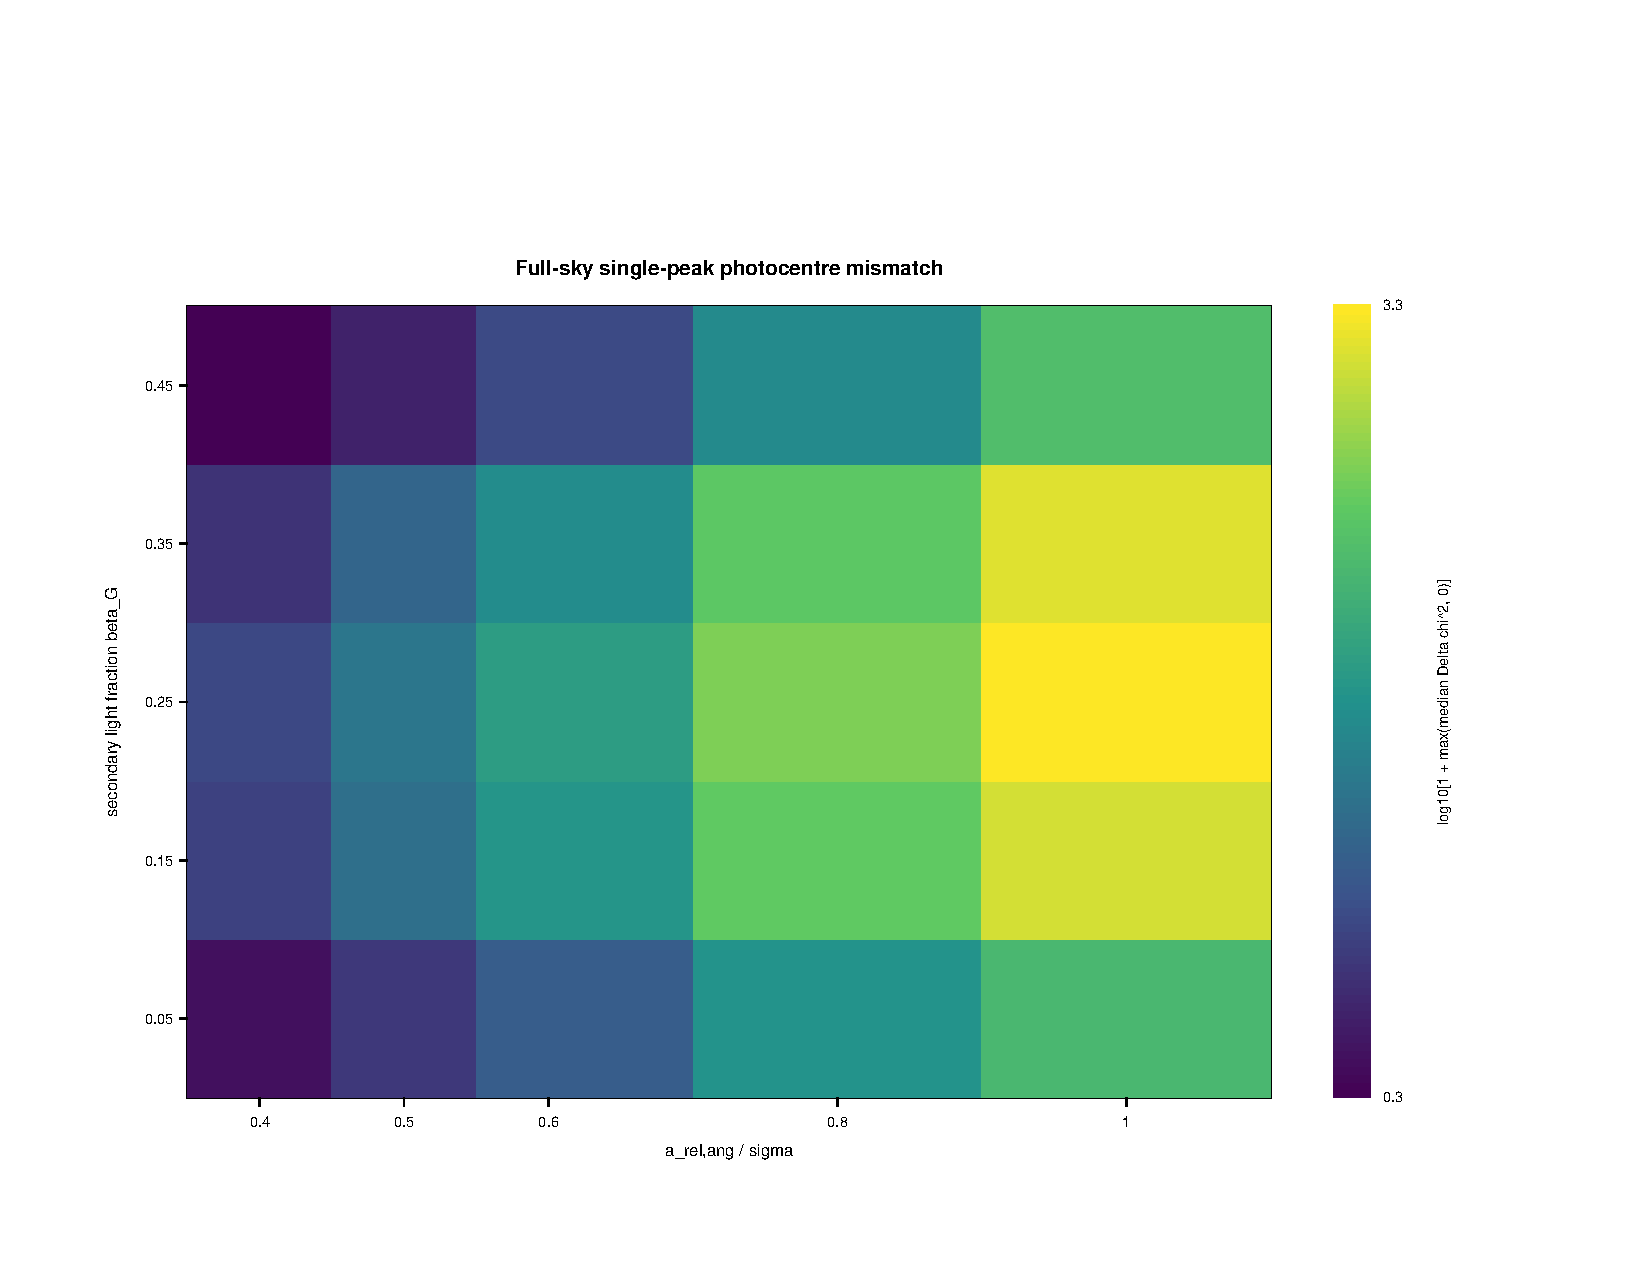
\includegraphics[width=0.92\textwidth]{figures/full_sky_dr4_beta_separation_surface}
\caption{Full-sky native-schedule photocentre--RAA mismatch in the single-peak domain. Each cell is the median paired $\dchi$ over all sky positions and noise seeds, displayed logarithmically. The surrogate width $\sigma$ is a research scale and the horizontal coordinate is not a Gaia resolution threshold.}
\label{fig:surface}
\end{figure}

\subsection{Full-Sky Variation}

At $\betag=0.25$ and $\asig=1$, the sky distribution of median $\dchi$ has minimum 834.14, median 2195.39, and maximum 8766.64. The native $Q_{16}(\dchi)>0$ boundary first occurs at the smallest sampled ratio, $\asig=0.40$, for 41/46 positions, while the remaining five first cross at 0.50. Requiring all ten realizations at a sky position to have $\dchi>0$ moves the first crossing to 0.40 for 18 positions, 0.50 for 23, and 0.60 for five. These are descriptive sampled boundaries rather than formal detection thresholds.

At the same $(\betag,\asig)$ point the Spearman rank correlation between median $\dchi$ and native transit count is
\begin{equation}
\rho_{\rm S}=0.7709.
\end{equation}
The corresponding correlations with maximum directional scan-angle gap and normalized directional entropy are $-0.640$ and $+0.358$, respectively. The native sky dependence therefore combines observation count and scan geometry.

\begin{figure}
\centering
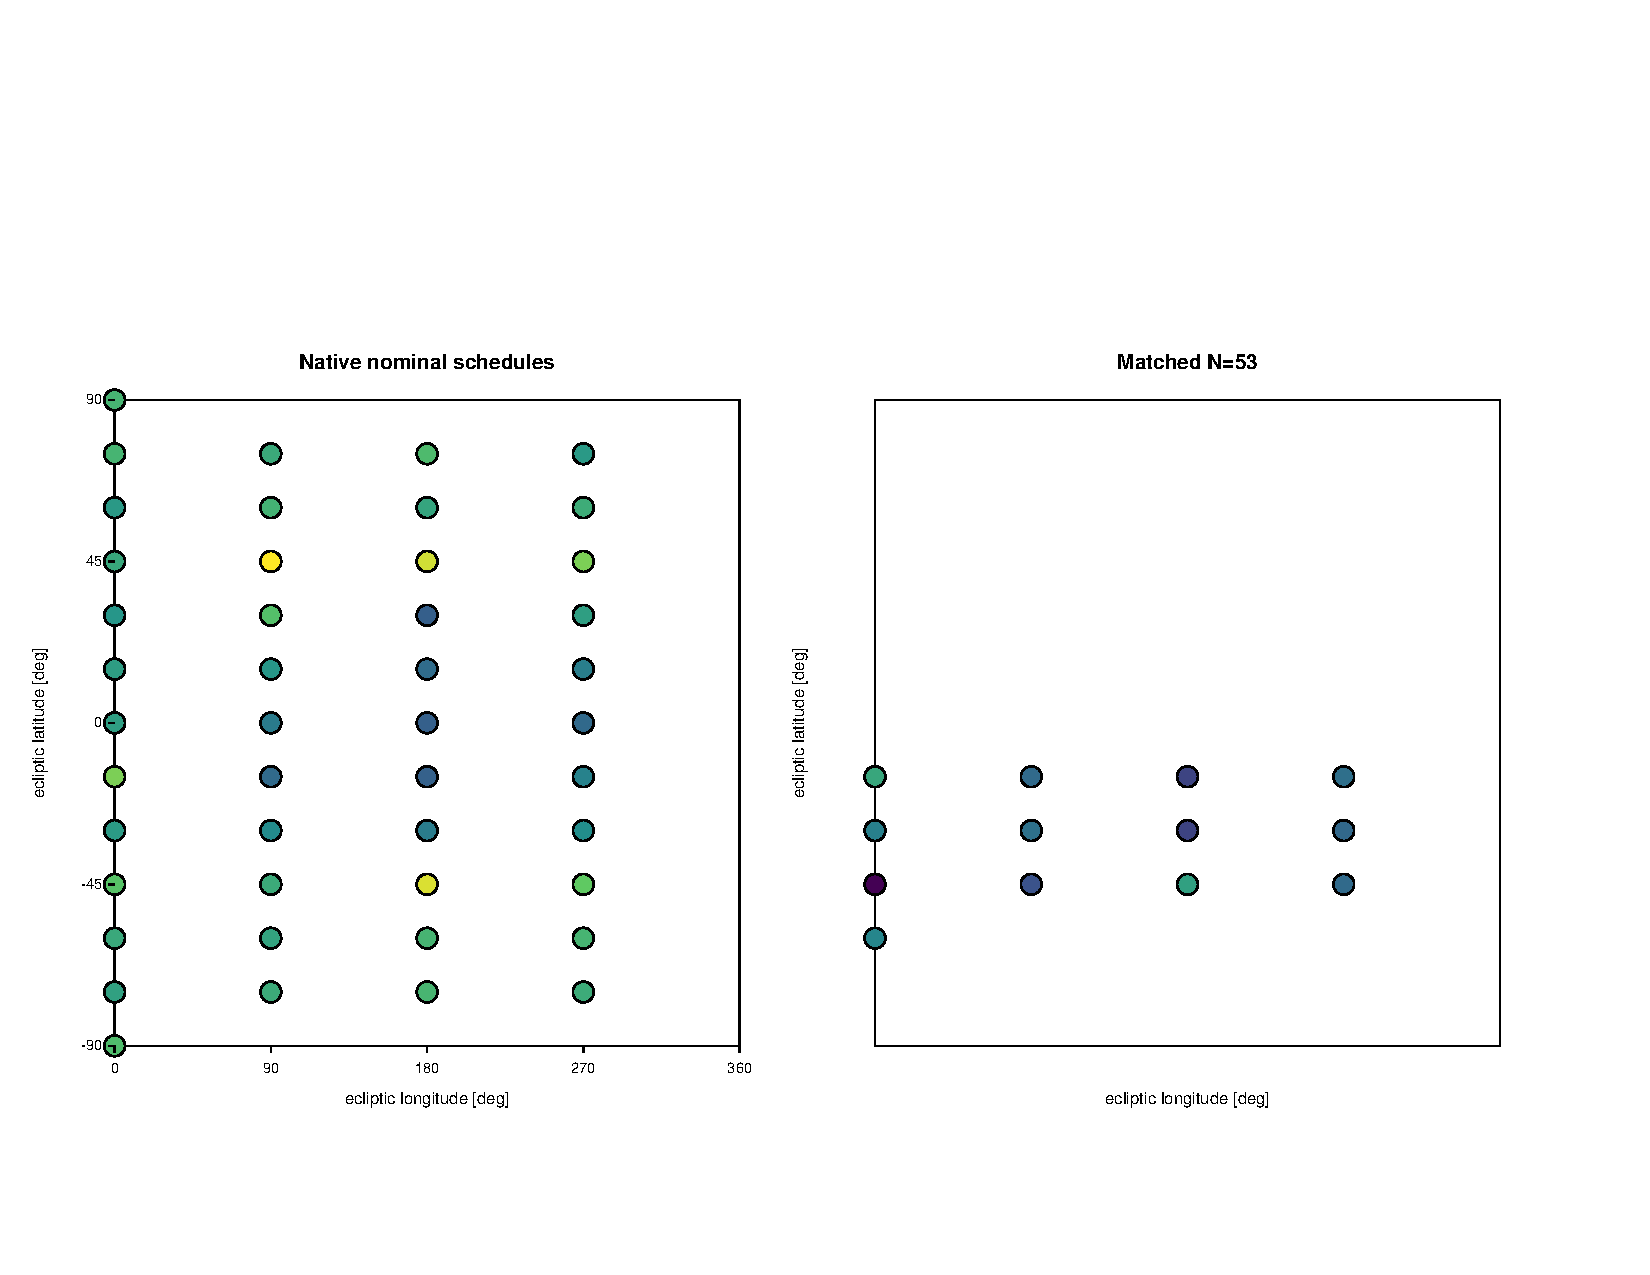
\includegraphics[width=0.98\textwidth]{figures/full_sky_dr4_native_matched_sky}
\caption{Sampled ecliptic-sky maps of the median paired $\dchi$ for $\betag=0.25$ and $\asig=1$, using the same logarithmic colour normalization. The left panel uses the native nominal schedules with 53--310 transits; the right panel uses the matched schedules with exactly 53 transits.}
\label{fig:skymaps}
\end{figure}

\subsection{Matched-Transit-Count Control}

Fixing all positions to $N=53$ reduces the sky-median $\dchi$ from 2195.39 to 1180.94, a ratio of 0.5379. The matched sky range is 300.04--2230.26, substantially narrower than the native 834.14--8766.64 range. Most importantly, the correlation with the \emph{native} transit count becomes
\begin{equation}
\rho_{\rm S}(\dchi_{53},N_{\rm native})=-0.0032,
\end{equation}
consistent with no monotonic relation. This shows directly that the strong native correlation was driven by the number of retained measurements rather than merely by another sky property correlated with $N$.

Figure~\ref{fig:nativecontrol} compares native and matched values at each sky position. High-$N$ native schedules generally move furthest below the one-to-one line when reduced to 53 measurements.

\begin{figure}
\centering
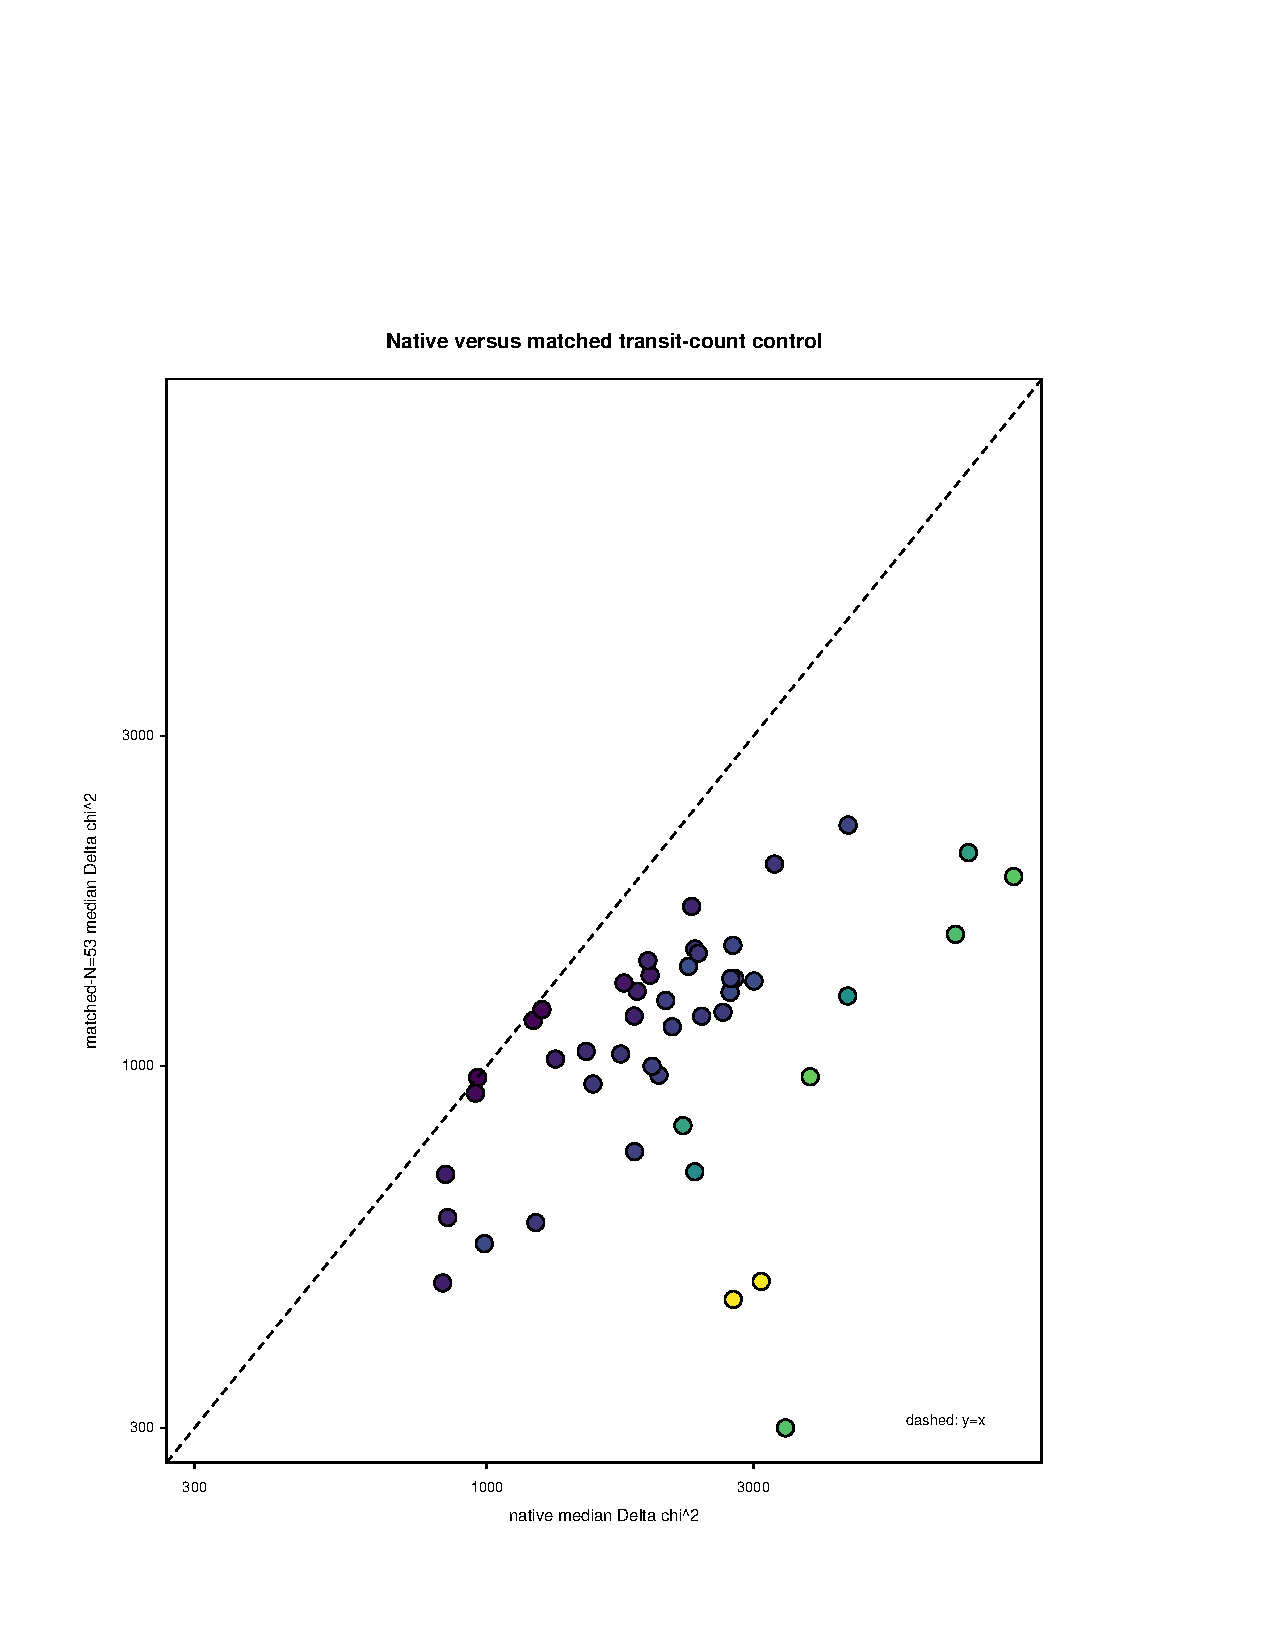
\includegraphics[width=0.80\textwidth]{figures/full_sky_dr4_native_vs_matched_n53}
\caption{Native versus matched-$N=53$ median $\dchi$ across the 46 sky positions for $\betag=0.25$ and $\asig=1$. Colour denotes the native nominal transit count. The dashed line is equality.}
\label{fig:nativecontrol}
\end{figure}

The ratio of model discrepancies closely follows the fraction of transits retained:
\begin{equation}
\rho_{\rm S}\left(
\frac{\dchi_{53}}{\dchi_{\rm native}},
\frac{53}{N_{\rm native}}
\right)=0.9233.
\end{equation}
Furthermore,
\begin{equation}
{\rm median}\left[
\frac{\dchi_{53}/\dchi_{\rm native}}{53/N_{\rm native}}
\right]=1.0138.
\label{eq:scaling}
\end{equation}
The median native discrepancy per transit is 21.44, compared with 22.28 in the matched control. Within this particular synthetic strong-response case, Equation~(\ref{eq:scaling}) is therefore consistent with an approximately linear accumulation of model-discrimination information with the number of Gaia-like observations.

\begin{figure}
\centering
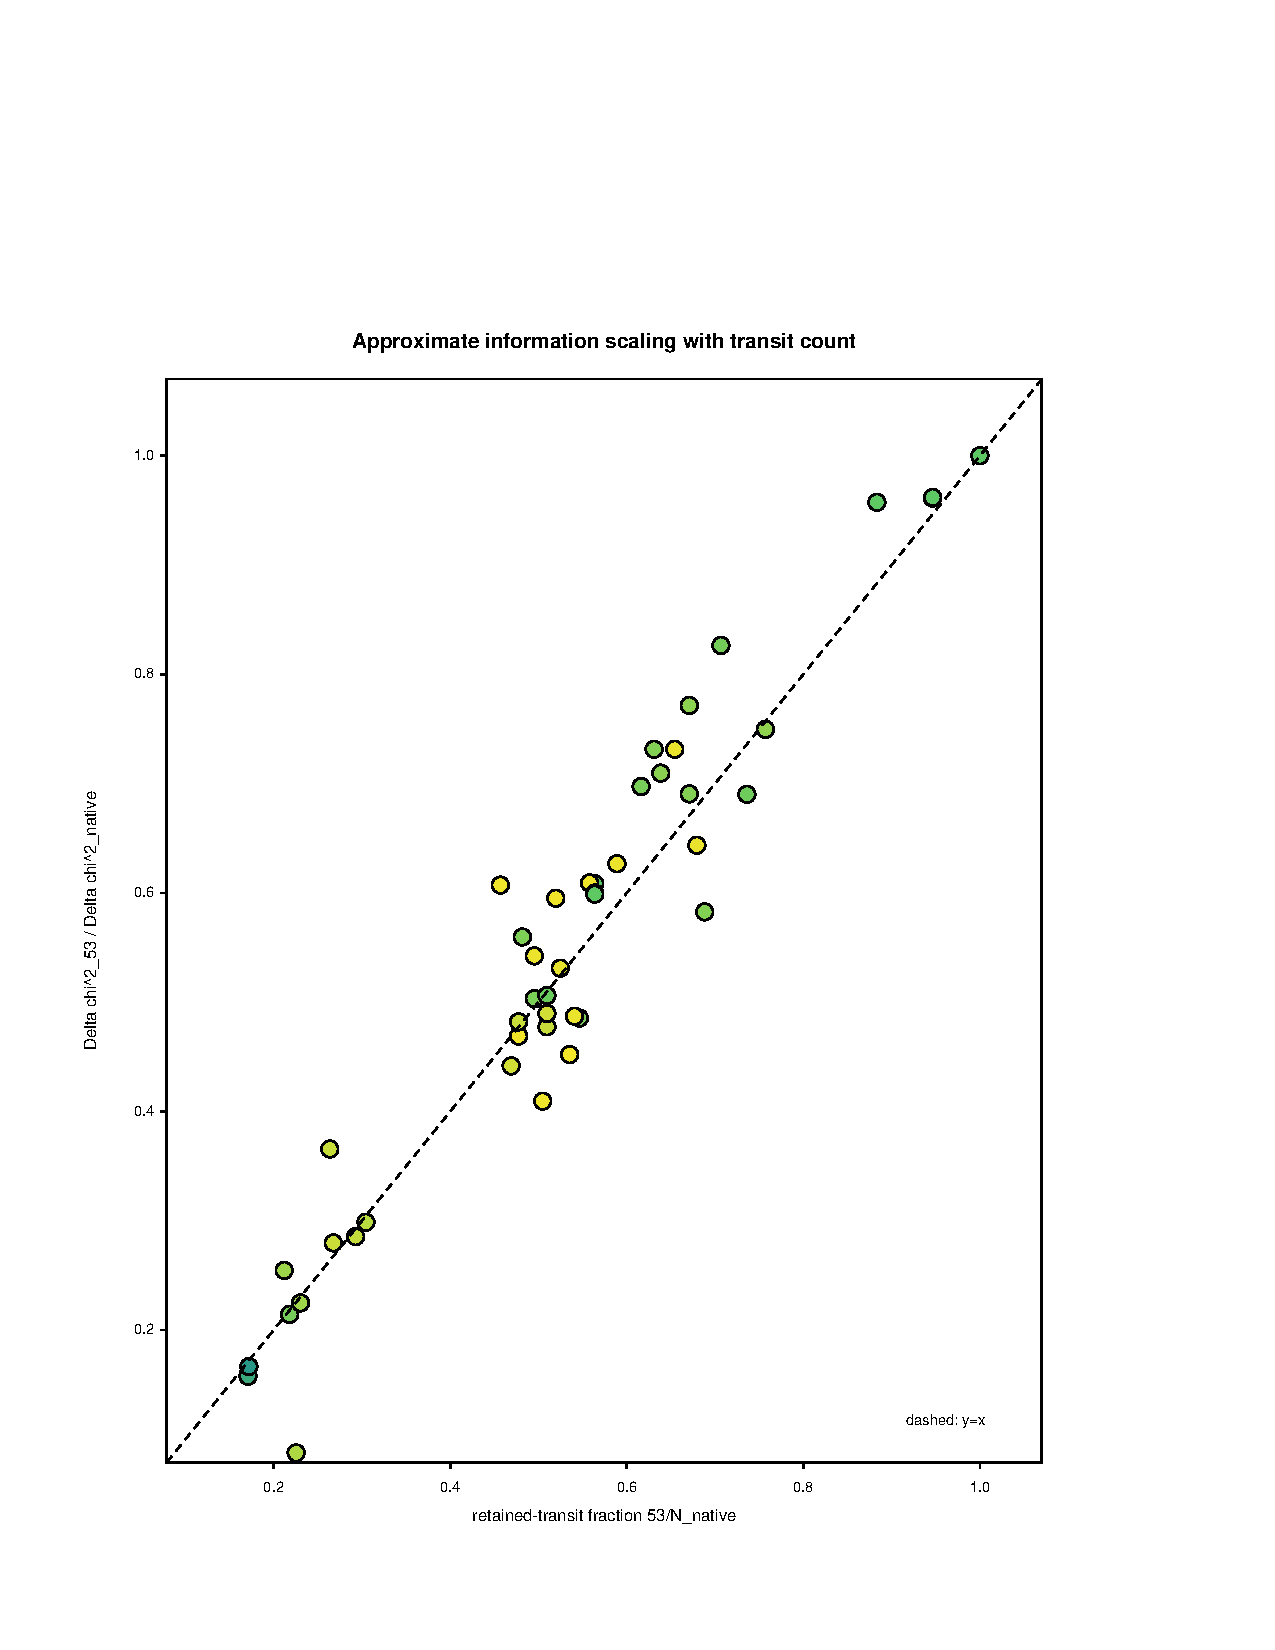
\includegraphics[width=0.80\textwidth]{figures/full_sky_dr4_matched_n53_scaling}
\caption{Ratio of matched to native model discrepancy versus the retained-transit fraction. Each point is one sky position at $\betag=0.25$ and $\asig=1$. The dashed line is the simple proportional scaling $\dchi_{53}/\dchi_{\rm native}=53/N_{\rm native}$; colour denotes the normalized scan-angle entropy of the 53 retained measurements.}
\label{fig:scaling}
\end{figure}

Equalizing the count does not erase all sky dependence. For the same control point, $\rho_{\rm S}(\dchi_{53},H_{\rm angle})=+0.340$ and $\rho_{\rm S}(\dchi_{53},\Delta\psi_{\max})=-0.275$, where $H_{\rm angle}$ is normalized directional entropy and $\Delta\psi_{\max}$ is the maximum directional angular gap. Thus scan geometry leaves a measurable residual contribution after the dominant count effect is removed.

The transition boundary shifts accordingly. At $\betag=0.25$, 31/46 matched positions have $Q_{16}(\dchi)>0$ by $\asig=0.40$ and 15/46 first cross at 0.50. For the stricter all-seeds-positive condition the matched first crossings are 0.40 for eight positions, 0.50 for 24, 0.60 for 13, and 1.00 for one position. Additional observations therefore move the descriptive transition inward for a substantial part of the sky.

\subsection{Bias in Physical Parameters}

The photocentre model can partially absorb a wrong measurement response by changing fitted physical parameters. Pooling all sky positions and seeds at $\asig=1$, the median fractional photocentre bias in $\betag$ is $-22.6\%$, $-18.0\%$, $-12.6\%$, $-7.17\%$, and $-2.12\%$ for $\betag=0.05,0.15,0.25,0.35,0.45$, respectively. For the central $\betag=0.25$ case, the median photocentre mass biases pooled over the full sky are approximately $-0.61\%$ for $M_1$ and $-0.66\%$ for $M_2$, while the median parallax bias is $+0.51\%$. Across individual sky positions, the median $\betag$ bias ranges from $-19.3\%$ to $-8.0\%$, whereas median mass biases remain within about $-1.6\%$ to $+0.9\%$.

This separation is informative: the parameter with the largest fractional bias need not coincide with the light fraction that maximizes $\dchi$. Model-discrimination strength and parameter-bias amplitude are distinct diagnostics.

\begin{table}
\begin{center}
\caption{Key Full-Sky and Matched-$N$ Results at $\betag=0.25$, $\asig=1$}
\label{tab:results}
\begin{tabular}{lcc}
\hline\noalign{\smallskip}
Quantity & Native schedules & Matched $N=53$\\
\hline\noalign{\smallskip}
Fit records in experiment & 23\,000 & 11\,040\\
Sky positions & 46 & 46\\
Transit count & 53--310 & 53\\
Sky min median $\dchi$ & 834.14 & 300.04\\
Sky median median $\dchi$ & 2195.39 & 1180.94\\
Sky max median $\dchi$ & 8766.64 & 2230.26\\
$\rho_{\rm S}(\dchi,N_{\rm native})$ & 0.7709 & $-0.0032$\\
$\rho_{\rm S}(\dchi,H_{\rm angle})$ & 0.358$^\dagger$ & 0.340\\
\noalign{\smallskip}\hline
\end{tabular}
\end{center}
\tablecomments{0.86\textwidth}{$^\dagger$Native value quoted for normalized directional entropy. All $\dchi$ values are descriptive paired model differences, not formal significance statistics.}
\end{table}

\section{Discussion}
\label{sect:discussion}

\subsection{What the Synthetic Experiment Establishes}

The central result is not merely that a two-Gaussian profile differs from its flux-weighted centroid. Rather, the joint inference shows a broad controlled regime in which the profile is still single-peaked, yet the peak coordinate is sufficiently non-photocentric that a full eleven-parameter orbit fit cannot remove the discrepancy without degrading the joint likelihood.

The light-fraction dependence is physically interpretable within the restricted surrogate. The effect vanishes toward a dark secondary because the second light profile disappears, and it vanishes toward exact equal-light symmetry in the single-peak limit because the central maximum and photocentre coincide. Intermediate light fractions maximize the displacement of the peak from the flux-weighted position. The fact that $\betag=0.25$ is the maximum at all 230 native sampled sky/separation combinations makes this behavior robust within the tested orbit and grid rather than a feature of one scan geometry.

The full-sky experiment also demonstrates why a single representative sky position is insufficient. The same binary parameters can produce order-of-magnitude changes in native $\dchi$ because Gaia's nominal cadence and directional sampling vary over the sky. The matched-$N$ experiment then shows that most of this large-scale variation is attributable to observation count: after all positions are reduced to 53 measurements, the correlation with native $N$ vanishes and the matched/native discrepancy ratio closely tracks the retained fraction. Residual correlations with scan-angle entropy and maximum gap show that geometry remains a secondary contributor.

\subsection{What the Experiment Does Not Establish}

Several limitations are deliberate and define the next tests.

First, the Gaussian width is a research scale for the baseline experiment. Neither $\sigma=50$ mas nor any sampled $\asig$ value is a calibrated Gaia resolution scale. The quantitative transition locations cannot be translated directly into angular separation criteria for real Gaia data.

Second, the baseline model uses the global maximum of a two-equal-width-Gaussian one-dimensional profile. This is a restricted case of the blended-source problem treated more generally by \citet{Penoyre2026}, who include an elongated PSF through an orientation-dependent effective width. The published correction to that work changes signs in several equations, and the corrected expressions must be used in the next implementation. Gaia itself uses a calibrated PLSF whose DR4 treatment includes drift-scan effects and dependences on source colour and focal-plane position \citep{Rowell2026}. Window assignment, gating, background, source matching, detection, and calibration effects are absent from the baseline surrogate.

Third, the schedules are nominal GOST-derived mission trajectories. They encode sky-position-dependent times and scan directions but not the exact source-level set of successful observations. The native full-sky study should therefore be interpreted as a controlled mission-geometry experiment, not a prediction of the number of usable epochs for a specific star.

Fourth, the synthetic study holds one physical orbit, noise prescription and external-data design fixed. Equation~(\ref{eq:scaling}) should not be generalized into a universal Gaia law $\dchi\propto N$ without tests over period, eccentricity, inclination, mass ratio, magnitude/noise, external astrometric precision, and orbit/scan phase relationships.

Finally, the frozen quantitative results use the deterministic eleven-parameter baseline fitter. The repository now also contains absolute-astrometric terms, a validation-grade posterior sampler, and response-misspecification controls, but those additions were made after the frozen experiments and are not retroactively part of the 23\,000- and 11\,040-fit result sets. Real target analyses will require a production posterior engine, the Gaia spacecraft ephemeris, and calibrated response/nuisance models.

\subsection{The Literature Gap After the Deeper Audit}

The candidate contribution has to be stated at the intersection of existing methods rather than as a new ingredient in isolation. Combined orbit inference from absolute astrometry, independent relative astrometry, and component-labelled radial velocities is established by BINARYS and related tools \citep{Brandt2021,Leclerc2023}. Indeed, \citet{Chevalier2023} already combined Gaia DR3 astrometric solutions with SB2 data to derive individual stellar masses and luminosities. Component-mass inference from unresolved Gaia astrometric orbits and photometry is also established \citep{BailerJones2026}. Neither Gaia+SB2 nor Gaia-derived component masses are novelty claims available to this work.

BINARYS nevertheless provides an unusually direct motivation for the remaining measurement problem. It models the non-trivial Hipparcos transit response when secondary light matters, but \citet{Leclerc2023} explicitly limit the analogous luminous partially resolved Gaia case because the flux contamination/LSF fitting cannot be reconstructed from the Gaia catalogue products then available. The published Gaia DR3 NSS processing likewise discarded partially resolved doubles before its orbital pipeline \citep{Halbwachs2023}. Our target regime is therefore a documented limitation of existing stellar processing rather than a regime invented for the synthetic experiment.

A physical nonlinear blended-source response is itself established. \texttt{gaiamock} implements the equal-width peak response reproduced by our baseline \citep{ElBadry2024}; its public source also contains a forward predictor that combines that response with a primary-star RV curve. Therefore even response-aware stellar Gaia+RV forward modelling cannot be claimed as new. The audited public path did not reveal the full target-level inverse combination pursued here, but absence from one code path is not proof of absence in the literature.

The Arecibo analysis removes another broader priority claim. \citet{Liu2024} fitted a binary asteroid using Gaia FPR astrometry with an unresolved/partially-resolved/resolved response and external occultation relative positions. Thus a partially resolved Gaia response has already been used inside orbital inference. That analysis is sequential, is not a stellar SB2, and has no pair of stellar RV curves; those distinctions define the remaining intersection rather than making the underlying response physics new.

Bayesian Gaia epoch-astrometry plus RV inference is established by \citet{Baycroft2026}. Public Octofitter code additionally provides epoch-level Gaia DR4 likelihood infrastructure alongside relative-astrometry and RV modules. In the specific public Gaia likelihood paths audited for this project, we did not identify a physical marginal-resolution blended-profile operator. The remaining \emph{candidate} gap is consequently very narrow: a stellar target-level inference in which that operator is fitted inside the Gaia epoch likelihood while the same dynamical model is simultaneously constrained by independent resolved relative astrometry and \emph{both} SB2 velocity curves, with response assumptions propagated into $M_1$, $M_2$, parallax, and light ratio. We make no priority claim for this exact intersection.

More importantly, the stronger scientific question is independent of software priority: \emph{how much dynamical-mass and parallax bias is caused by treating marginal-resolution Gaia measurements as an ordinary photocentre, and what fidelity of response model is required to recover calibrated inference?} That question is the reason to continue the project even if another implementation eventually occupies the same capability intersection.

\subsection{Response Fidelity as the Decisive Test}

The matched-surrogate baseline gives the resolution-aware model an intentional advantage: the response used in the fit is exactly the response used to generate the Gaia-like data. The next experiment must remove that advantage. We therefore define a response hierarchy on the same synthetic observations: $M_0$ is the ordinary photocentre, $M_1$ is the equal-width Lindegren/\texttt{gaiamock}-family peak response, and $M_2$ is an orientation-dependent response based on the corrected effective-width treatment of \citet{Penoyre2026}. A later $M_3$ should allow response parameters to vary as nuisance parameters rather than asserting them.

The principal diagnostics should then be the fractional biases
\[
\frac{\widehat M_1-M_{1,\rm true}}{M_{1,\rm true}},\qquad
\frac{\widehat M_2-M_{2,\rm true}}{M_{2,\rm true}},\qquad
\frac{\widehat\varpi-\varpi_{\rm true}}{\varpi_{\rm true}},
\]
and the empirical coverage of nominal 68 and 95 per cent posterior intervals. $\dchi$ remains a useful model-mismatch diagnostic, but a large residual preference is scientifically less important than whether the inferred masses are accurate and the posterior intervals are calibrated.

The combined visual-SB2 design also creates an identifiability opportunity. The two RV amplitudes strongly constrain the mass ratio, while resolved astrometry constrains the relative orbit. Such a system can therefore provide an externally constrained projected component separation at each Gaia epoch. In principle, the remaining mapping from that separation to the measured Gaia coordinate can be used to constrain response nuisance parameters. An ensemble of well-measured visual SB2s may therefore serve as an empirical calibrator of Gaia's close-pair response rather than merely as targets whose masses require correction.

\subsection{Gaia DR4 Opportunity and Overlap Risk}

The official Gaia DR4 expected-content table already lists provisional products directly relevant to this programme, including \texttt{epoch\_astrometry}, \texttt{epoch\_image}, and \texttt{rvs\_epoch\_data\_double}. The table is explicitly under development and subject to processing and validation changes, and the detailed DR4 processing documentation/final data model are not yet released. These are therefore official expected product names, not guessed interfaces.

This is simultaneously the main opportunity and the largest remaining novelty blind spot. The public material reviewed here does not establish whether the eventual DPAC NSS likelihood internally uses a physical marginal-resolution PLSF/image response for orbital inference. Until the DR4 processing papers and documentation are available, we should claim neither that DPAC does nor that it does not implement such an inversion.

The planned \texttt{epoch\_image} product points to the natural long-term extension. Once a blended profile becomes genuinely multi-peaked, collapsing a transit to one astrometric coordinate is no longer a robust measurement model. An image/sample-domain likelihood would model the CCD samples directly and eliminate the need for an artificial single-coordinate continuation through that regime.

Until suitable epoch/image products are public, DR3 catalogue diagnostics can provide only indirect consistency tests. Quantities such as \texttt{ipd\_frac\_multi\_peak} and \texttt{ipd\_gof\_harmonic\_amplitude} are qualitatively related to partially resolved structure, but they include Gaia detection, windowing, calibration, and IPD behaviour and should not be equated directly with the mode count or residuals of the present surrogate.

\section{Conclusions}
\label{sect:conclusion}

We developed a physically constrained joint orbit prototype for resolved relative astrometry, SB2 radial velocities, and Gaia-like along-scan measurements with a resolution-aware single-peak response. The main conclusions are:

\begin{enumerate}
\item The baseline equal-width response recovers the ordinary photocentre in the unresolved limit but admits a distinct single-peak, non-photocentric regime before mode splitting. The response is not new: it reproduces the published \texttt{gaiamock} response \citep{ElBadry2024} and is a restricted case of the broader treatment of \citet{Penoyre2026}.
\item Neither combined Gaia/relative-astrometry/SB2 fitting nor Gaia-based component-mass inference is new \citep{Leclerc2023,Chevalier2023,BailerJones2026}; nor is response-aware orbital inference in general, as demonstrated for Arecibo \citep{Liu2024}.
\item The surviving candidate methodological gap is the specific stellar inverse combination: a physical marginal-resolution operator inside an epoch Gaia likelihood, fitted simultaneously with independent resolved relative astrometry and both SB2 velocity curves and propagated to individual masses. We make no priority claim for this intersection.
\item Explicit orbit conventions and single/multi-peak validity checks are essential; internally self-consistent synthetic recovery alone is insufficient to detect orientation-convention errors.
\item Across 23\,000 native full-sky baseline fits, $\betag=0.25$ gives the largest median photocentre--RAA discrepancy at all 230 tested sky/separation combinations.
\item At $\betag=0.25$ and $\asig=1$, the native sky-median $\dchi$ is 2195.39; matching every sky position to 53 observations reduces it to 1180.94 and removes the native correlation with transit count.
\item The matched/native discrepancy ratio tracks the retained-transit fraction with $\rho_{\rm S}=0.923$, while residual scan-angle dependence remains.
\item These values characterize a restricted matched-surrogate synthetic design; they are not physical Gaia resolution thresholds, empirical Gaia calibration results, or evidence that the same advantage survives realistic response misspecification.
\item The decisive next question is therefore response fidelity: whether progressively more realistic response models improve mass/parallax bias and posterior coverage when the injected measurement physics is deliberately not identical to the fitted model.
\end{enumerate}

The longer-term observational programme is to use DR4 epoch astrometry and, eventually, epoch images to test the same hierarchy on real visual SB2s and to determine whether strong external orbital constraints can empirically calibrate the close-pair astrometric response.

\section*{Data and Code Availability}

The implementation, validation tests, analysis scripts, compact frozen result tables, and manuscript figures are versioned in the accompanying \texttt{RAA\_Orbit\_Model} repository. The large raw synthetic CSV files are generated by the documented scripts; the committed frozen tables contain the numerical summaries used in this manuscript. Exact nominal scan schedules are archived by the experiment runner so that the same directional sampling can be re-used without re-querying the scanning-law provider.

\begin{acknowledgements}
The author acknowledges the open Gaia mission documentation and the public software and literature resources used to construct the controlled scanning-law experiments.
\end{acknowledgements}


\bibliographystyle{raa}
\bibliography{raa_orbit_refs}

\label{lastpage}
\end{document}
